\section{Randomised particle generation}
\label{section:randomised-particle-generation}

For our particle generation, we rely on the convex hull algorithm
\cite{mattutis,3,5}.
We place 50 points random on the unit sphere
They act as input to the computation of a convex hull which yields around 60
triangles typically.
Each vertex of the resulting mesh then is scaled with a random scalar from
$[0.75,1]$.
Thus, we obtain distorted particles that do not resemble a sphere and can be
slightly convex.
The resulting mesh is finally suitably dilated and scaled.

\begin{figure}[htb]
  \begin{center}
    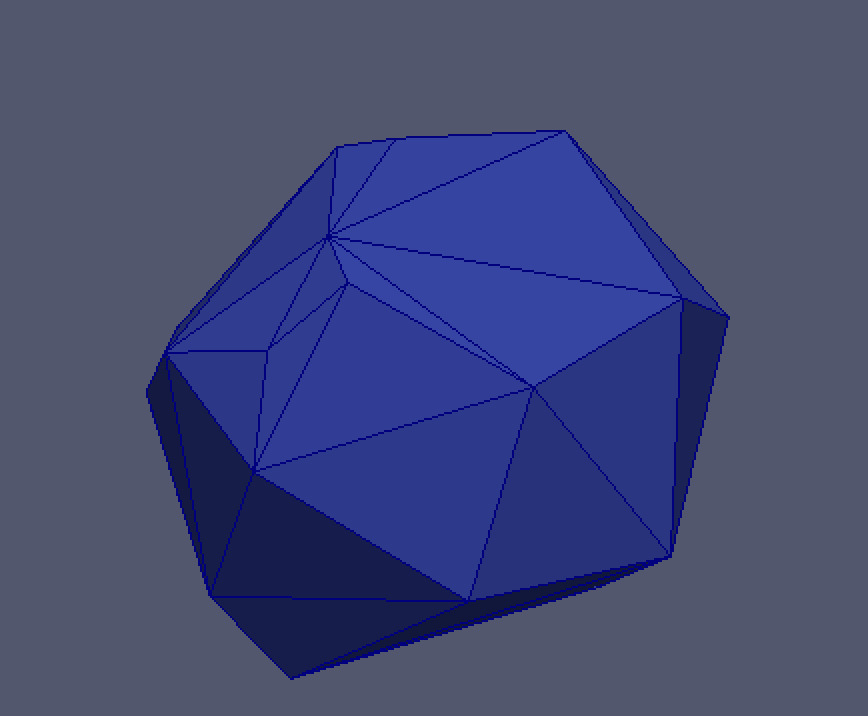
\includegraphics[width=0.5\textwidth]{sketches/coarse.png}
  \end{center}
  \caption{Coarse non-spherical particle triangulation using Hull and Delaney algorithm.}
  \label{figure:coarse_particle}
\end{figure}

\begin{figure}[htb]
  \begin{center}
    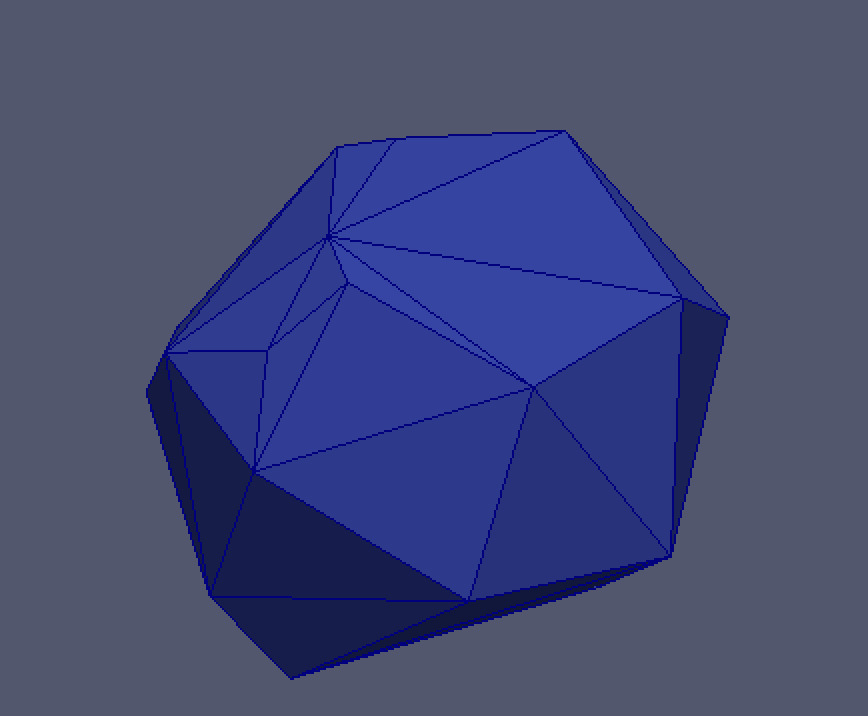
\includegraphics[width=0.5\textwidth]{sketches/coarse.png}
  \end{center}
  \caption{Fine spherical particle triangulation using Hull and Delaney algorithm.}
  \label{figure:fine_particle}
\end{figure}


\marginpar{\footnotesize KK: Can you please add here two or three pictures from
typical particles?}
